\documentclass[../Main.tex]{subfiles}

\begin{document}
\chapter{Information Theory / Coding}

\intro{

}

\section{Information Theory}
\begin{figure}
    \centering
    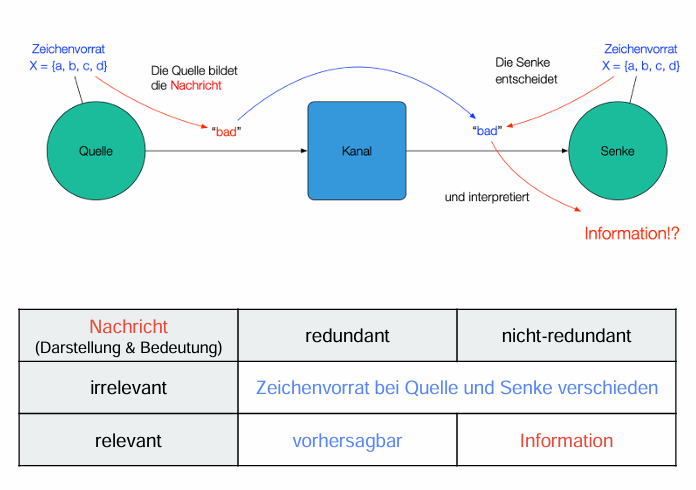
\includegraphics[width=0.5\linewidth]{Images/information.png}
    \caption{Information Theory Term Overview}
    \label{fig:it-term-overview}
\end{figure}

\defn{Decision Content / Entscheidungsgehalt}{
    The measure of the effort required to form a message or to decide on a decision of a message is the decision content.
    \begin{equation}
        H_0 = log_2(N)[\text{bit}]
    \end{equation}
}

\defn{Decision Flow / Entscheidungsfluss}{
    The formula measures the rate of information flow necessary to make a decision over time.
    \begin{equation}
        H_0 = \frac{log_2(N)}{\tau}
    \end{equation}
    Where \( \tau \) is the time required for the transmission of a word.
}

\defn{Information Content}{
    The information content of a sign indicates how many elementary decisions have to be made to determine this sign.
    \begin{equation}
        I(x_k)=log_2(\frac{1}{P(x_k)})
    \end{equation}
}


\defn{Entropy (mittlerer Informationsgehalt)}{
    Entropy is the average information content of the source. It therefore shows how many elementary decisions the source/sink has to make on average per character
    \begin{equation}
        H(X) = \sum_{k=1}^{N} P(x_k) \cdot I(x_k) = \sum_{k=1}^{N} p(x_k) \cdot log_2(\frac{1}{P(x_k)})
    \end{equation}

    Since we typically use a binary encoding for the discrete values of the source we use:

    \begin{equation}
        \begin{split}
            &L(X)=\sum_{k=1}^{N} P(x_k) \cdot I_r(x_k) \\
            &\text{where } I_r = I(x_k) \text{ aufgerundet (auch tatsächliche Codewortlänge)}
        \end{split}
    \end{equation}
}

\defn{Source Redundancy (Redundanz der Quelle)}{
    \begin{equation}
        R_Q = H_0 - H(X)
    \end{equation}
}

\defn{Prefix Code}{
    A prefix code is a code that fulfills the Fano condition: No code word of the code is a prefix of another code word. In other words, no code word may be the beginning of another code word. For example, a code with the code words \{0, 10, 11\} fulfills the prefix property, whereas the code with the code words \{0, 01, 10\} does not, as 0 is the prefix of 01.
}

\thm{Shannons Theorem}{
     Für jede beliebige zugehörige Binärcodierung mit Präfixeigenschaft ist die mittlere Codewortlänge nicht kleiner als die Entropie \( H(X) \).

     \begin{equation}
         H(x) \leq L
     \end{equation}

     Für jede beliebige Quelle kann eine Binärcodierung gefunden werden, so dass die folgende Ungleichung gilt:
     \begin{equation}
         H(X) \leq X \leq H(X) + 1
     \end{equation}
}

\defn{Code Redundancy}{
    \begin{equation}
        R_C = L - H(X)
    \end{equation}
}

\defn{Discrete Source with and without memory}{
    Die mittlere Entropie einer Quelle ohne Gedächtnis ist stets grösser oder gleich der Entropie einer Quelle mit Gedächtnis. In der Quellencodierung sind daher nicht Einzelzeichen zu codieren, sondern stets Zeichenketten.
    \begin{equation}
            R_Q = H_0 - H_{oG}(X) \leq H_= - H_{mG}(X)
    \end{equation}
}

\section{Huffman}
Verfahren zur Entwicklung eines kommafreien Codes mit minimaler mittlerer Codewortlänge Rekursives Verfahren, d.h. der Binärbaum wird nicht von der Wurzel, sondern von den Blättern aus entwickelt

%\exm{Algorithm}{
%    \begin{enumerate}
%        \item Ordne die Zeichen gemäss ihrer Auftrittswahrscheinlichkeit
%        \item Die beiden Zeichen mit der kleinsten Auftrittswahrscheinlichkeit haben die gleiche CW-Länge \( L_N \)
%        \item Sei \( L_N \) die mittlere CW-Länge für eine Quelle mit \( N \) Zeichen und \( L_{N-1} \) die mittlere CW-Länge für den Fall, dass die beiden letzten zu einem einzigen Zeichen zusammengefasst werden, dann gilt:
%        \begin{equation}
%            
%        
%            \begin{split}
%                L_N - (P(x_{N-1}) + P(x_N)) \cdot L(x_N) &= L_{N-1} - (P(x_{n-1}) P(x_N)) \cdot L(X_N)-1 \\
%                &\Rightarrow L_N = L_{N-1} + P(x_{N-1})+P(x_N)
%            \end{split} 
%        \end{equation}
%    \end{enumerate}
%    \begin{figure}
%        \centering
%        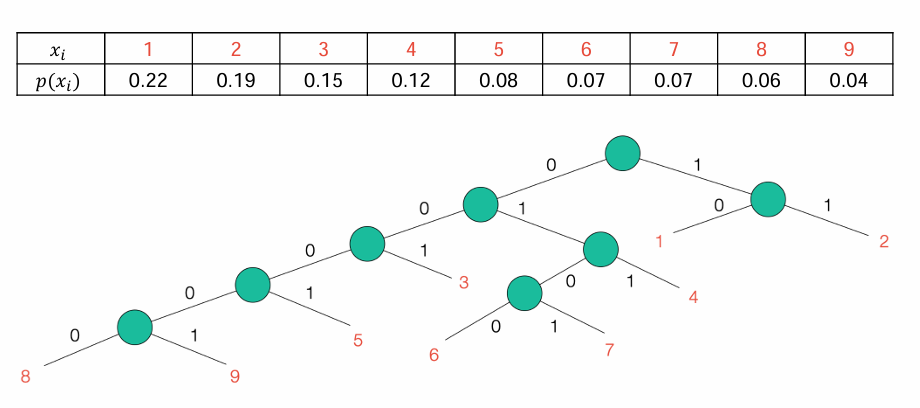
\includegraphics[width=0.5\linewidth]{Images/huffman.png}
%        \caption{Huffman Example}
%        \label{fig:huffman-example}
%    \end{figure}
%}

\section{Lempel-Ziv}
\exm{Algorithm}{
    \begin{enumerate}
        \item Suche in der Tabelle eine möglichst lange Zeichenfolge, die mit den nächsten \(N\) zu kodierenden Zeichen übereinstimmt.
        \item Bilde ein Token und speichere es.
        \item Verschiebe das Fenster um \( N+1 \) Zeichen.
        \item Wiederhole, bis alle Zeichen kodiert sind.
    \end{enumerate}
}

\section{Kanalmodell}
TODO

\end{document}
